%!TEX encoding = UTF-8 Unicode

%!TEX root = ../compendium.tex

\Lab{\LabWeekNINE}

\begin{Goals}
\item Kunna skapa och iterera över matriser med nästlade for-loopar.
\item Kunna använda sig av och förstå arv.
\item Förstå och träna på olika villkor med if-satser.
\item Känna till algoritmer för att lösa problem så som att ta sig igenom en labyrint eller slumpmässigt skapa en labyrint
\end{Goals}

\begin{Preparations}
\item Läs om matriser.
\item Läs om arv.
\item Läs om olika algoritmer för att ta sig igenom en labyrint: \\
(\href{https://en.wikipedia.org/wiki/Maze\_solving\_algorithm})
\item Läs om olika sätt att skapa en slumpmässig labyrint: \\
(\href{https://en.wikipedia.org/wiki/Maze\_generation\_algorithm}).
\item Läs om olika algoritmer för att ta sig igenom en labyrint
\end{Preparations}

\subsection{Bakgrund}
I denna laboration kommer du att få skapa labyrinter och sedan implementera algoritmer för att ta dig igenom dessa. En labyrint är ett rum som har en ingång och en utgång. Ingången är i de här fallen alltid längst ner i labyrinten, och utgången högst upp. Alla väggar är också parallella med antingen x-axeln eller y-axeln. Ett sätt att beskriva en sådan labyrint i kod är med hjälp av en matris. Varje element i matrisen motsvarar då en ``ruta'' i labyrinten. Värdet TRUE representerar att det finns en vägg och FALSE representerar att det är fri väg att gå där.

Det finns många olika sätt att ta sig igenom en labyrint men ett av de vanligaste och enklaste sätten att konstruera en algoritm är att hålla sin vänstra hand mot den vänstra väggen och gå framåt utan att släppa väggen med handen tills man når slutet av labyrinten. Detta funkar för alla labyrinter där väggarna från ingången till utgången är sammankopplade.

\subsubsection{Den frivilliga uppgiften}
I den frivilliga uppgiften ska en slumpmässig labyrint genereras. Det finns flera olika algoritmer för att göra detta men den vi kommer använda här är en slumpmässig variant av Prims algoritm. Du kan läsa mer under \url{https://en.wikipedia.org/wiki/Maze\_generation\_algorithm} (De representerar en labyrint på ett annat sätt än vi gör i den här uppgiften vilket innebär att det inte kommer se precis likadant ut). 

\subsection{Obligatoriska uppgifter}

\Task I denna uppgift ska du implementera en metod som kan rita upp en labyrint i SimpleWindow.

\Subtask Läs igenom klassen Maze och se till att du förstår det mesta. Vad Maze gör är att den läser in rader med strängar, antingen från en fil eller direkt som argument, där tecknet '\#' representerar en vägg och ' ' representerar en gång. Utifrån detta skapar Maze en Boolean-matris ``mapMatrix'' som representerar labyrinten, där TRUE står för vägg och FALSE står för gång. Fråga om något är oklart!

\Subtask Implementera metoden DRAW i Maze som ritar upp labyrinten i SimpleWindow. För att göra detta behöver du gå ingenom matrisen "mapMatrix" i Maze och undersöka elementen på varje plats. Om ett element är TRUE så betyder det att det här ska finnas (det vill säga ritas upp) en vägg i labyrinten, om FALSE att det här ska finnas en gång. Ta hjälp av metoden brickInTheWall som finns tillgänglig i Maze-klassen.

\Task En labbuppgiftsbeskrivning.

\Subtask Skapa en ny klass AMazeIngRace genom att välja File -> New -> Scala Class. I denna klass ska du skriva en main-metod där du skapar ett objekt av klassen Maze genom att läsa in från fil (börja exempelvis med filen maze1.txt). Du måste även skapa ett objekt av SimpleWindow för att skicka med i draw-metoden. Anropa sedan metoden draw på Maze-objektet och kolla att labyrinten ritas upp som den ska. Gör samma sak för resterande av filerna mazeX.txt, alla ska kunna ritas upp korrekt. Testa att rita en egen labyrint genom att skapa en textfil och lägg i samma mapp som övriga maze-filer. Kontrollera så att även denna ritas upp som den ska, och fixa annars till metoden draw så att den fungerar som tänkt.

\Task I den här uppgiften ska du implementera en algoritm för att få en sköldpadda att ta sig genom en labyrint med hjälp av att alltid hålla i väggen med vänster hand (eller kanske fot i det här fallet!).

\Subtask Skapa en ny klass MazeTurtle som ärver från klassen ColourTurtle. MazeTurtle ska ta ett extra argument, nämligen ett av typen Maze som är den labyrint som sköldpaddan ska gå i.

\Subtask Definiera i MazeTurtle en ny metod "walk". Implementera sedan denna metod. I metoden ska sköldpaddan med hjälp av tekniken "hålla vänster hand i väggen" ta sig genom labyrinten, från början till slut. Varje steg motsvarar att flytta sig från en ruta till en annan i Boolean-matrisen i Maze. Sköldpaddan kommer alltså ta sig fram genom att undersöka för varje steg om den borde svänga vänster, det vill säga om den inte har någon vägg till vänster om sig längre, om den borde gå rakt fram eller om den borde svänga höger.

\Subtask Lägg till kod i AMazeIngRace som skapar en sköldpadda och sedan låter denna gå igenom labyrinten med metoden walk. Testa att din MazeTurtle fungerar som den ska! Sköldpaddan ska klara att ta sig igenom alla labyrinter i filerna maze1.txt - maze3.txt samt din egna labyrint.

\subsection{Frivilliga extrauppgifter}
Prims algoritm är ett sätt att hitta hur man kopplar ihop alla punkterna i en graf med så få kopplingar som möjligt. Detta låter nog som rena grekiskan men tänk dig att punkterna är varje ruta i labyrinten och en hopkoppling är där du kan gå vilket innebär två öppna rutor intill varandra. Eftersom algoritmen vill ha så få kopplingar som möjligt får inga ``rundor'' uppstå utan det kommer endast finnas en väg igenom labyrinten

I praktiken funkar algoritmen genom att den väljer en slumpmässig ruta intill en öppen ruta och kollar om det är någon mer öppen ruta intill. Om så är fallet låter den rutan vara en vägg annars öppnar den rutan. Den upprepar detta tills alla rutor antingen öppnats eller låtit vara en vägg.

Eftersom det endast ska finnas en in- och utgång måste detta hanteras på lite annats sätt.
\begin{enumerate}
	\item Börja med att välja en av rutorna i botten och öppna den och rutan över.
	\item Applicera ovanstående algoritm på alla rutor utom de rutor som är runt (Så att vi får en vägg som går runt hela).
	\item Efteråt letar vi efter en slumpmässig ruta på näst översta raden som är öppen och öppnar rutan ovanför.
\end{enumerate}

\begin{figure}[h]
	\begin{center}
		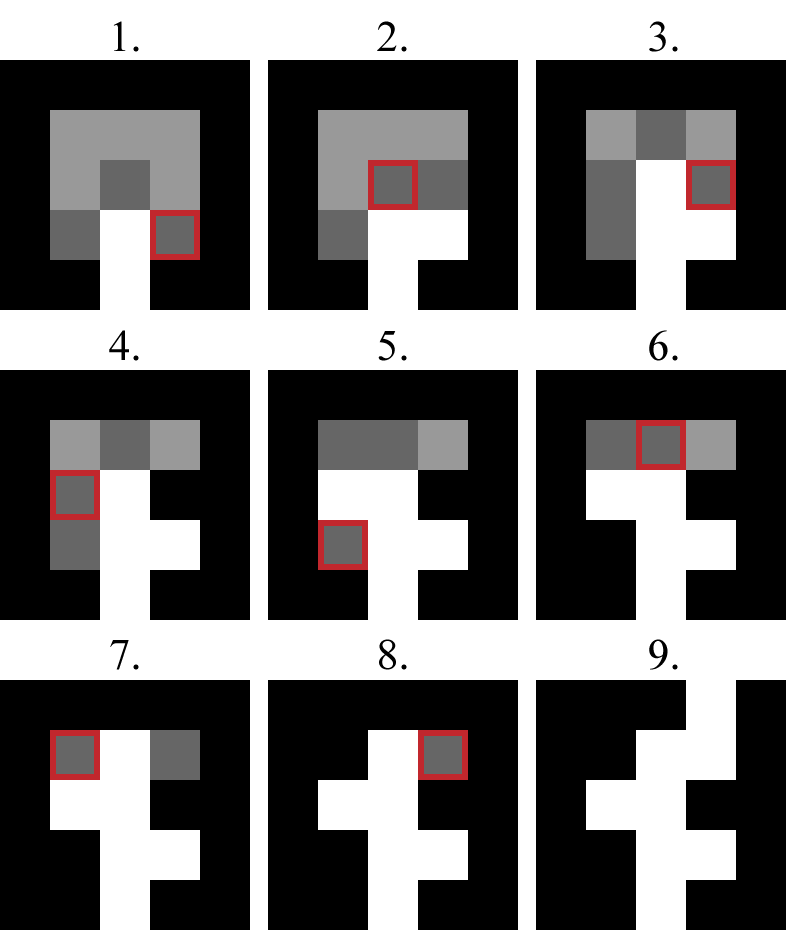
\includegraphics[width=0.45\textwidth]{../img/w09-lab/AlgorithmVisualized.png}
	\end{center}
	\caption{Visualisering av algoritmen när den genererar en labyrint av storleken 5x5}
\end{figure}

\subsubsection{Psuedokod}
\begin{Code}
def random(rows, cols)
	labyrint = matris(rows, cols) fylld med true
	buffer = lista(koordinater till rutor)
	
	Välj en slumpmässig ruta i nedersta raden och öppna den
	
	Öppna rutan ovanför
	Lägg till rutorna runt till buffern
	
	while(buffer har element kvar)
		element = välj slumpmässigt element i buffer
		if (element har max en öppen ruta intill sig)
			öppna rutan element innehåller
			lägg till rutorna runt till buffern
		ta bort element från buffer
	
	Hitta en ruta som är öppen i näst översta raden
	Öppna rutan ovanför
\end{Code}

%Börja med att välja en slumpmässig kolumn som startkolumn och den nedersta raden som startrad ur matrisen
%Markera i matrisen att platsen (startrad)(startkolumn) och platsen (startrad - 1)(startkolumn) i "brädet" inte är en vägg (då det är ingången!)
%Lägg till platsen (startrad - 1)(startkolumn) i listan med väggar
%Så länge som listan med väggar inte är tom:
%    Välj ett slumpmässigt tal (index) mellan 0 och storleken på listan med väggar
%    Hämta det element (row, col) som finns på platsen index i listan med väggar
%    Om det finns väggar runt omkring platsen (row, col):
%        Markera i matrisen att platsen (row, col) inte är en vägg
%        Lägg till platsen (row)(col) i listan med väggar
%    Ta bort elementet på plats index i listan med väggar
%Sätt en variabel check till false
%Så länge check är sann
%    Välj ett slumpmässigt tal X mellan 0 och antalet kolumner
%    Om elementet på plats i matrisen (1)(X) inte är en vägg
%        Markera i matrisen att (0)(X) inte är en vägg
%        Sätt check till att inte vara sann
%Skapa en ny labyrint med matrisen som inparameter


%    Start with a grid full of walls.
%    Pick a cell, mark it as part of the maze. Add the walls of the cell to the wall list.
%    While there are walls in the list:
%        Pick a random wall from the list. We now have two cases: either there exists exactly one unvisited cell on one of the two sides of the chosen wall, or there does not. If it is the former:
%            Make the wall a passage and mark the unvisited cell as part of the maze.
%            Add the neighboring walls of the cell to the wall list.
%        Remove the wall from the list.


\Task I den här uppgiften ska du implementera en algoritm för att skapa en slumpmässig labyrint.

\Subtask Inspektera ovanstående pseudokod och försök förstå den. Fråga gärna om något är oklart! Läs också de färdigskrivna metoderna i metoden "random" i Maze och se om du kan förstå vad de gör.

\Subtask Implementera metoden random i Maze som skapar och returnerar en slumpmässigt utformad labyrint med hjälp av "pseudokoden" ovan (eller på egen hand för den modiga/nyfikna!). Ta även hjälp av de färdigskrivna metoderna addWallsToBuffer och checkWallsAround.

\Subtask Skapa en ny labyrint i AMazeIngRace genom att anropa din random-metod! Vad får du för resultat? Ett bra värde att använda på storleken när du anropar metoden är mellan 50 och 100. Dvs anropa metoden med till exempel random(50, 50). Om du lyckas få fram en labyrint och din random-metod är korrekt, testa att låta sköldpaddan gå igenom labyrinten och se vad som händer!
    
